\documentclass[12pt]{article}
\usepackage{lecture}
\usepackage{html}
\usepackage{graphicx}
\usepackage{epstopdf}
\usepackage[
  bookmarks=true,
  bookmarksopen=true,
  pdftitle={Getting started with {\tt R}},
  pdfauthor={Kent E. Holsinger}]{hyperref}

\newcommand{\copyrightYears}{2021}

\makeindex  

\title{Getting started with {\tt R}}

\begin{document}

\maketitle

\tableofcontents

\section{Introduction}

We will be using the freely available statistical programming package
{\tt R}  extensively during this course. In fact, we'll use a software
package other than {\tt R} only when I can't find a way to do it in
{\tt R}. As a result, you'll be quite familiar with {\tt R} by the end
of the course, which you will find very useful even if you never use
anything else you learn in this course. Because of the very large
number of add-on packages available for {\tt R}, virtually any
statistical analysis you'd ever want to do will have a package
available for it in {\tt R}.\footnote{If you happen to be a devotee of
  {\tt Python}, none of what I just said is intended to deprecate {\tt
    Python}. Much of what I just wrote about {\tt R} could also be
  written about {\tt Python}, but for the time being {\tt R} is more
  widely used for statistical analysis than {\tt Python}. That may
  change before long. Even now, my impression is that people who work
  in bioinformatics and genomics increasingly use {\tt Python} rather
  than {\tt R} for many of their day-to-day tasks.}

\subsection{Installing {\tt R}}

Installing {\tt R} is fairly straightforward. Point your browser to
CRAN, the Comprehensive {\tt R} Archive Network:
\url{https://cran.r-project.org/}. At the top of the page you'll see
download links for Linux, MacOS, and Windows. Pick the appropriate
link, and download the latest release, which you'll find at the top of
the page. Install it using the standard approach for your machine, and
you should be all set.

\subsection{Installing {\tt RStudio}}

If you were to click on the {\tt R} icon that should show up on your
machine now, you'd see something like the screenshot in
Figure~\ref{fig:R-screenshot}.\footnote{You'll probably see a couple
  of differences from what's displayed here. You probably won't see
  the error message in red type, and you'll probably see a version
  number larger than 4.0.2.}

\begin{figure}
  \begin{center}
    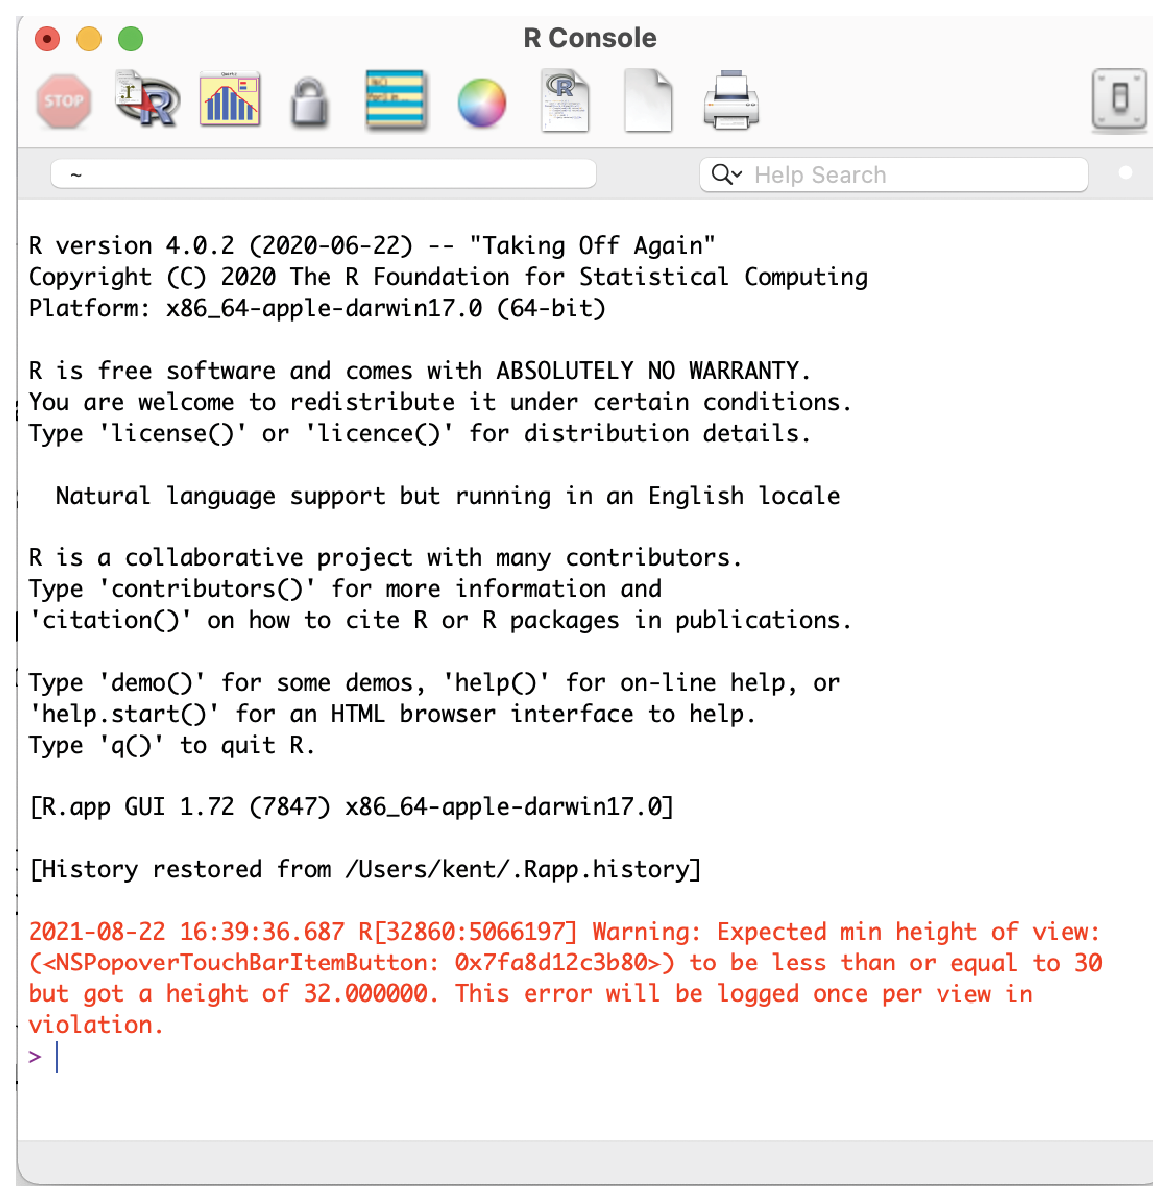
\includegraphics[width=10cm]{R-screenshot.eps}
  \end{center}
  \caption{A screenshot of the {\tt R} console.}\label{fig:R-screenshot}
\end{figure}

\noindent That ``$>$'' at the bottom of the screen is a command
prompt. That's where you'd enter commands, and {\tt R} would
respond. You can certainly work with {\tt R} directly from the
console. That's what I did until a couple of years ago. Then I finally
broke down and took the advice of several colleagues and
students\footnote{My students have always been a lot smarter than I
  am.} and installed {\tt RStudio}. Now I almost never work from the
{\tt R} console, except through the console window in {\tt RStudio}.

To install {\tt RStudio} simply visit
\url{https://www.rstudio.com/products/rstudio/download/#download},
click on {\tt Download} under {\tt RStudio Desktop}, and download the
version of {\tt RStudio} appropriate for your machine. Install it
following the procedures you normally use and you're all set.

\section{Getting started}

\subsection{Working with {\tt RStudio}}

Now that you have {\tt RStudio} installed, click on its icon. When you
do, you'll see something like Figure~\ref{fig:RStudio}

\begin{figure}
  \begin{center}
    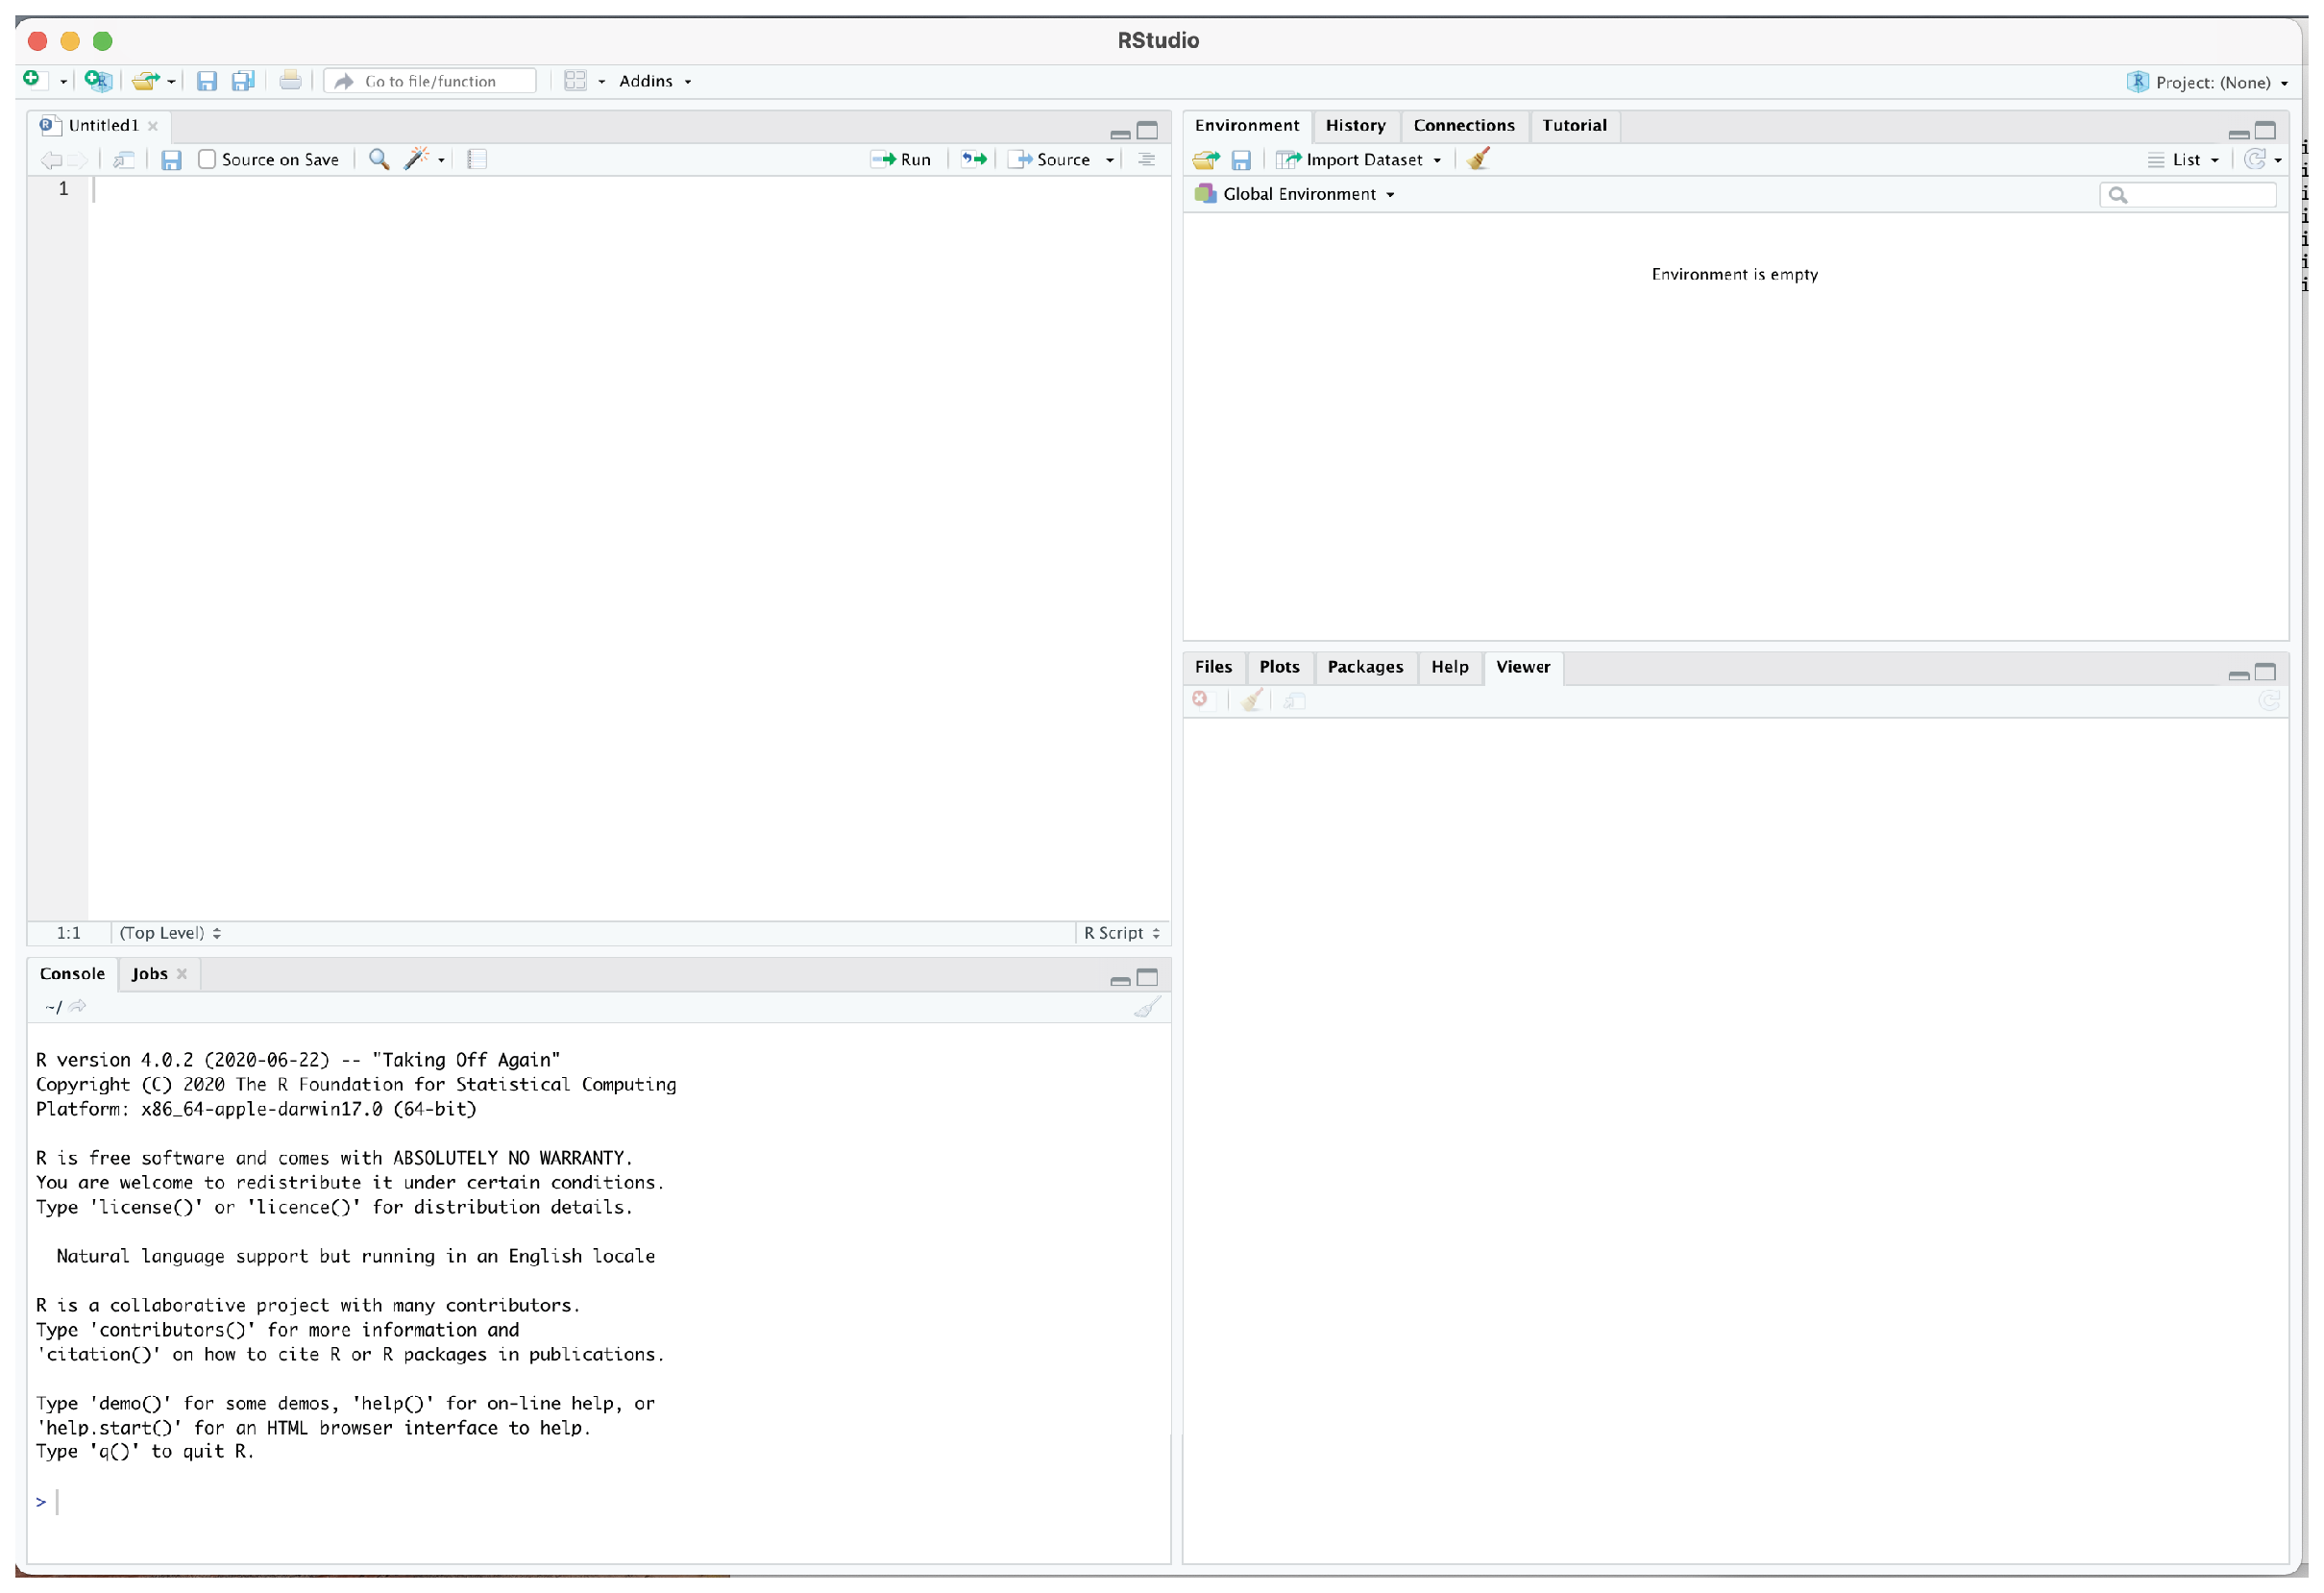
\includegraphics[width=16cm]{RStudio.eps}
  \end{center}
  \caption{The default {\tt RStudio} workspace.}\label{fig:RStudio}
\end{figure}
  
\noindent Right now it doesn't look like much, but that will change
soon.

I recommend that you create a directory on your machine where you can
store data files and other materials, but don't create it just
yet. Decide {\it where\/} you want to create it, then pull down the
file menu and select ``New project...'', then select the ``New
Directory'' option, then select ``New Project'', then choose a name
for the directory where your data and other materials will live, enter
it in the ``Directory name'' field, and use the ``Browse'' function to
find the directory within which this new directory will live. Click
create and {\tt RStudio} will create the directory and set up a few
files to keep it happy.\footnote{If you already have a directory you
  want to use pick the ``Existing directory'' option and use the
  ``Browse'' function to navigate to it.}

Once you're there I recommend that you do one more thing. Open up the
Preferences pane in {\tt RStudio}. Check ``Restore most recently
opened project at startup'' and ``Restore previously open source
documents at startup''. Those options mean that the next time you open
{\tt RStudio} you'll find yourself back in the directory you were
working in with any files you were working on open too.

\subsection{Installing packages}

For the time being, expand the lower right window so that it fills the
whole left side of your workspace by clicking the square in the far
upper right corner of the lower right window. That makes the console
window (the same console you saw in the screenshot of {\tt R} before)
occupy the whole left side of the window so that you can see more of
what's going on.

As I mentioned, one of the greath strengths of {\tt R} is the enormous
number of packages that allow you to do many different things. We'll
see only a tiny fraction of them in this course, but if you're ever
wondering how to do something in {\tt R}, Google is your friend. There
are a tremendous number of resources that can help you get your work
done.

We'll start by installing three packages that I use very frequently. I
won't dwell on what functions are in them. I'll just load them when I
need them, and use a few of the functions they provide. Here's all you
need to do. At the command prompt enter each of the following lines
and wait for your computer to stop churning. If it asks about
installing any of the packages from source, respond with an ``N''.

\begin{verbatim}
install.packages("tidyverse")
install.packages("readxl")
install.packages("ggplot2")
\end{verbatim}

You may get a message asking you to select a mirror. If you do, scroll
through the list until you find something in the US and pick one that
appeals to you. All of the mirrors have the same set of packages. They
differ only in that some are closer than others.

\subsection{Getting data into {\tt R}}

Now that you've installed those packages we're ready to get
started. Download the file {\tt isotoma.csv} at
\url{http://darwin.eeb.uconn.edu/eeb348-resources/isotoma.csv} and
save it in the directory you're using to store data and files for this
lab. Now type

\begin{verbatim}
library(tidyverse)
\end{verbatim}

\noindent You'll see a message that some packages are being attached
and that there are some conflicts. Don't worry about the
conflicts. They aren't things you need to worry about\footnote{Until you're an
advanced {\tt R} user. Then you'll what they mean, and you'll know how
to handle the conflict if it's ever necessary to do so.} This command
makes the functions in the {\tt tidyverse} package available. Without
it, those functions aren't available even though they've been
installed.\footnote{To be completely honest I just lied, but what I
  said is close enough to the truth that by the time you know {\tt R}
  well enough to know how I lied, you won't need my help any more.}

Now we're ready to load the data we just downloaded into {\tt
  R}. Simply type

\begin{verbatim}
dat <- read_csv("isotoma.csv")
\end{verbatim}

\noindent You can probably guess what's going on here, but let's walk
through it slowly.

\begin{itemize}

\item {\tt read\_csv("isotoma.csv")} - {\tt read\_csv()} is a function
  that reads a file with comma separated values, a CSV
  file. "isotoma.csv" is the name of the file we want to
  read.\footnote{If you've used {\tt R} before, you'll probably know
    that there's also a {\tt read.csv()} function. It works much the
    same as {\tt read\_csv()}, but {\tt read\_csv()} behaves a bit more
    nicely.}

\item The function stores its result in a data object named {\tt
    dat}. We could have given the object any name, like {\tt wally}
  for example, but it's best to pick names that are reasonably
  descriptive and easy to remember.

\end{itemize}

\noindent If you've been paying {\it very\/} close attention to your
workspace, you'll notice that in the upper right window there's now
something that says {\tt dat}. To the right of that you'll see a
statement that there are 188 observations of 2 variables. If you click
on {\tt dat}, you'll see a window open in the upper left of your
workspace that looks like a spreadsheet with 2 columns (the variables)
and 188 rows (the observations). You'll see these data again when we
get to $F$-statistics next week. For now simply notice that each row
describes the genotype of an individual plant. The first column is the
population from which the plant was collected, and the second column
is the genotype at a particular locus, $GOT-1$, where 2 refers to one
homozygote, 1 to the heterozygote, and 0 to the other
heterozygote. {\tt dat} is an example of what we call a ``data
frame'' in {\tt R}.

\section{Lab exercise \#1}

\begin{itemize}

  \item You can get a list of all of the values in the column of a
    data frame by typing the name of the data frame followed
    immediately by \$ and followed immediately again the the name of
    the column whose values you want to see.

    Try it with {\tt dat\$pop}.

  \item You can find out how many unique values there are in a list
    with {\tt unique()}.

    How many different populations are there in the {\it Isotoma}
    data set? Show me the {\tt R} code you used to get the answer.

  \item You can count the number of times each unique value occurs
    in a list with {\tt table()}.

    How many individuals were collected from each population of {\it
      Isotoma}? Show me the {\tt R} code you used to get the answer.

  \item You can select a subset of rows from a data frame that meet
    a particular criterion with {\tt subset()}. Use {\tt
      help(subset)} to see the internal help on using {\tt subset()}
    in {\tt R} and Google further if that doesn't help.
    
    Construct a new data frame (using {\tt subset()} consisting of
    individuals from Boora. Using that data frame count the number of
    individuals of each genotype (0, 1, 2), and estimate the genotype
    and allele frequency. Show me the {\tt R} code you used to get the
    answer.

\end{itemize}

\section{Additional resources on {\tt R}}

Here are a few additional resources on {\tt R} that you may find
useful if you need some additional help or want to begin digging
deeper.

\begin{itemize}

  \item {\tt R} tutorial for beginners from Datacamp:
    \url{https://www.statmethods.net/r-tutorial/index.html}

  \item {\tt R} tutorial from W3Schools:
    \url{https://www.w3schools.com/r/default.asp}

  \item A guide to {\tt R} tutorials from {\tt R-bloggers}:
    \url{https://www.r-bloggers.com/2015/12/how-to-learn-r-2/} 

\end{itemize}

\section{Acknowledgments}

These notes were inspired by a set of notes that Nora Mitchell
prepared when she was a teaching assistant in this course in 2017.

\ccLicense

\end{document}
